\documentclass[11pt,preprint, authoryear]{elsarticle}

\usepackage{lmodern}
%%%% My spacing
\usepackage{setspace}
\setstretch{1.2}
\DeclareMathSizes{12}{14}{10}{10}

% Wrap around which gives all figures included the [H] command, or places it "here". This can be tedious to code in Rmarkdown.
\usepackage{float}
\let\origfigure\figure
\let\endorigfigure\endfigure
\renewenvironment{figure}[1][2] {
    \expandafter\origfigure\expandafter[H]
} {
    \endorigfigure
}

\let\origtable\table
\let\endorigtable\endtable
\renewenvironment{table}[1][2] {
    \expandafter\origtable\expandafter[H]
} {
    \endorigtable
}


\usepackage{ifxetex,ifluatex}
\usepackage{fixltx2e} % provides \textsubscript
\ifnum 0\ifxetex 1\fi\ifluatex 1\fi=0 % if pdftex
  \usepackage[T1]{fontenc}
  \usepackage[utf8]{inputenc}
\else % if luatex or xelatex
  \ifxetex
    \usepackage{mathspec}
    \usepackage{xltxtra,xunicode}
  \else
    \usepackage{fontspec}
  \fi
  \defaultfontfeatures{Mapping=tex-text,Scale=MatchLowercase}
  \newcommand{\euro}{€}
\fi

\usepackage{amssymb, amsmath, amsthm, amsfonts}

\def\bibsection{\section*{References}} %%% Make "References" appear before bibliography


\usepackage[round]{natbib}

\usepackage{longtable}
\usepackage[margin=2.3cm,bottom=2cm,top=2.5cm, includefoot]{geometry}
\usepackage{fancyhdr}
\usepackage[bottom, hang, flushmargin]{footmisc}
\usepackage{graphicx}
\numberwithin{equation}{section}
\numberwithin{figure}{section}
\numberwithin{table}{section}
\setlength{\parindent}{0cm}
\setlength{\parskip}{1.3ex plus 0.5ex minus 0.3ex}
\usepackage{textcomp}
\renewcommand{\headrulewidth}{0.2pt}
\renewcommand{\footrulewidth}{0.3pt}

\usepackage{array}
\newcolumntype{x}[1]{>{\centering\arraybackslash\hspace{0pt}}p{#1}}

%%%%  Remove the "preprint submitted to" part. Don't worry about this either, it just looks better without it:
\makeatletter
\def\ps@pprintTitle{%
  \let\@oddhead\@empty
  \let\@evenhead\@empty
  \let\@oddfoot\@empty
  \let\@evenfoot\@oddfoot
}
\makeatother

 \def\tightlist{} % This allows for subbullets!

\usepackage{hyperref}
\hypersetup{breaklinks=true,
            bookmarks=true,
            colorlinks=true,
            citecolor=blue,
            urlcolor=blue,
            linkcolor=blue,
            pdfborder={0 0 0}}


% The following packages allow huxtable to work:
\usepackage{siunitx}
\usepackage{multirow}
\usepackage{hhline}
\usepackage{calc}
\usepackage{tabularx}
\usepackage{booktabs}
\usepackage{caption}


\newenvironment{columns}[1][]{}{}

\newenvironment{column}[1]{\begin{minipage}{#1}\ignorespaces}{%
\end{minipage}
\ifhmode\unskip\fi
\aftergroup\useignorespacesandallpars}

\def\useignorespacesandallpars#1\ignorespaces\fi{%
#1\fi\ignorespacesandallpars}

\makeatletter
\def\ignorespacesandallpars{%
  \@ifnextchar\par
    {\expandafter\ignorespacesandallpars\@gobble}%
    {}%
}
\makeatother

\newenvironment{CSLReferences}[2]{%
}

\urlstyle{same}  % don't use monospace font for urls
\setlength{\parindent}{0pt}
\setlength{\parskip}{6pt plus 2pt minus 1pt}
\setlength{\emergencystretch}{3em}  % prevent overfull lines
\setcounter{secnumdepth}{5}

%%% Use protect on footnotes to avoid problems with footnotes in titles
\let\rmarkdownfootnote\footnote%
\def\footnote{\protect\rmarkdownfootnote}
\IfFileExists{upquote.sty}{\usepackage{upquote}}{}

%%% Include extra packages specified by user

%%% Hard setting column skips for reports - this ensures greater consistency and control over the length settings in the document.
%% page layout
%% paragraphs
\setlength{\baselineskip}{12pt plus 0pt minus 0pt}
\setlength{\parskip}{12pt plus 0pt minus 0pt}
\setlength{\parindent}{0pt plus 0pt minus 0pt}
%% floats
\setlength{\floatsep}{12pt plus 0 pt minus 0pt}
\setlength{\textfloatsep}{20pt plus 0pt minus 0pt}
\setlength{\intextsep}{14pt plus 0pt minus 0pt}
\setlength{\dbltextfloatsep}{20pt plus 0pt minus 0pt}
\setlength{\dblfloatsep}{14pt plus 0pt minus 0pt}
%% maths
\setlength{\abovedisplayskip}{12pt plus 0pt minus 0pt}
\setlength{\belowdisplayskip}{12pt plus 0pt minus 0pt}
%% lists
\setlength{\topsep}{10pt plus 0pt minus 0pt}
\setlength{\partopsep}{3pt plus 0pt minus 0pt}
\setlength{\itemsep}{5pt plus 0pt minus 0pt}
\setlength{\labelsep}{8mm plus 0mm minus 0mm}
\setlength{\parsep}{\the\parskip}
\setlength{\listparindent}{\the\parindent}
%% verbatim
\setlength{\fboxsep}{5pt plus 0pt minus 0pt}



\begin{document}



\begin{frontmatter}  %

\title{Question 3}

% Set to FALSE if wanting to remove title (for submission)




\author[Add1]{Ronan Morris}
\ead{22876634}





\address[Add1]{Stellenbosch University}



\vspace{1cm}





\vspace{0.5cm}

\end{frontmatter}

\setcounter{footnote}{0}



%________________________
% Header and Footers
%%%%%%%%%%%%%%%%%%%%%%%%%%%%%%%%%
\pagestyle{fancy}
\chead{}
\rhead{}
\lfoot{}
\rfoot{\footnotesize Page \thepage}
\lhead{}
%\rfoot{\footnotesize Page \thepage } % "e.g. Page 2"
\cfoot{}

%\setlength\headheight{30pt}
%%%%%%%%%%%%%%%%%%%%%%%%%%%%%%%%%
%________________________

\headsep 35pt % So that header does not go over title




\hypertarget{portfolio-construction}{%
\section{Portfolio Construction}\label{portfolio-construction}}

I began this question by perusing the ZAR/USD exchange rate, and
searching periods with the highest volatility. This would result in
volatile years (defined as years with ZAR volatility that placed in the
top 3rd of all years' volatility) and low volatility years (measured as
years with a ZAR volatility in the bottom third of the rankings). The
high volatility years were 2016, 2018, 2020, and 2023. The low
volatility years were 2014, 2015, 2017, 2021.

I decided I would shade the years as red (high vol) and green (low vol)
on all ggplot objects created from the portfolio returns in this
question. This allowed a seamless discussion not only on how different
methodologies compared to one another, across cap sizes or whether the
funds or uncapped; it also allowed for a discussion about how these
funds and assets respond to volatility in the rand.

Figure 3.1 shows the 3-year rolling returns of the J403 and the J203
from 2013 until 2023. This plot only shows the returns for large cap
stocks. I would argue that - though these funds are not particularly
volatile - we see that during high volatility years, there is often dips
to the rolling returns, and sometimes these are quite drastic. One would
presume that large cap stocks are less exposed to huge fluctuations than
less supported stocks. The fund methodologies perform similarly over the
time period for large cap stocks, but I would mention that there are
times that the J203 experiences higher highs, but also marginally lower
lows, such as end of 2015 followed by later 2016.

\begin{figure}[H]

{\centering 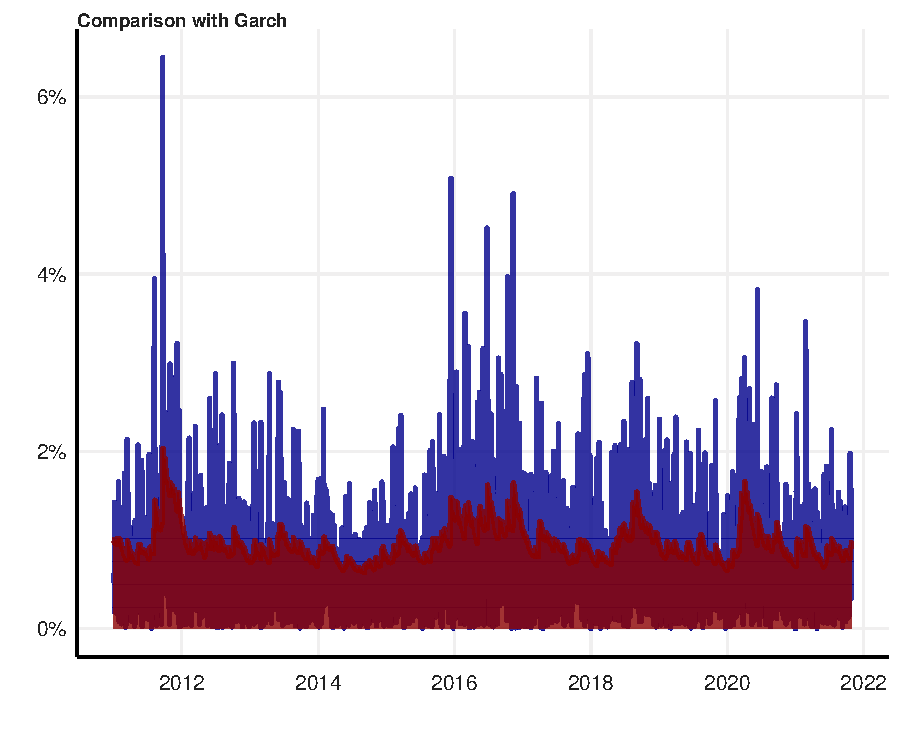
\includegraphics{Question-3_files/figure-latex/unnamed-chunk-1-1} 

}

\caption{Large Cap Stocks \label{Figure3.1}}\label{fig:unnamed-chunk-1}
\end{figure}

The plot of the 3 year rolling returns of mid cap shares in figure 3.2
exhibits more volatility. We see clear spikes and troughs during 2016
and 2020, with a sharp decline also present in 2018, though this is of a
similar size to troughs in 2015, which was a low volatility year for the
rand. What is of note here is that the rolling returns for the J203 and
J403 for mid cap shares is almost identical at each point.

\begin{figure}[H]

{\centering \includegraphics{Question-3_files/figure-latex/unnamed-chunk-2-1} 

}

\caption{Mid Cap Stocks \label{Figure3.2}}\label{fig:unnamed-chunk-2}
\end{figure}

The methodologies once again perform similarly in terms of 3 year
rolling returns for small cap stocks in figure 3.3. The small caps also
show extreme spikes in 2016 and lows in 2020, which are branded as high
volatility years. Similarly there is a downturn in 2018 and very small
returns in 2023.

\begin{figure}[H]

{\centering \includegraphics{Question-3_files/figure-latex/unnamed-chunk-3-1} 

}

\caption{Small Cap Stocks \label{Figure3.3}}\label{fig:unnamed-chunk-3}
\end{figure}

Next I applied capping to each of the J203 and J403, with the ALSI
capped at 10\% and the SWIX capped at 5\%. The cumulative returns for
this are shown in figure 3.4. The re-balancing was performed by using
the effective dates in the data set provided over the time period
discussed. The ggplot object is once again shown with high volatility
and low volatility time periods in order to further the discussion. In
the context of the full J203 and J403, with cumulative returns, the
volatility discussion becomes clear. The capped performance seems to
benefit the ALSI, considering that from around 2017 it steadily
outperforms the SWIX. We see that both steadily climb during the
``green'' years into 2016, were there is a plateau. They climb once more
in 2017 just to be stopped in 2018, and show extreme decreases during
2020, and a slowdown after climbing during low volatility years
preceding 2023.

\begin{figure}[H]

{\centering \includegraphics{Question-3_files/figure-latex/unnamed-chunk-4-1} 

}

\caption{ \label{Figure3.4}}\label{fig:unnamed-chunk-4}
\end{figure}

When we compare the uncapped portfolio returns, we see that the ALSI
takes longer to overtake the SWIX, but it still eventually does. This
implies that the ALSI stands to benefit more from the capping procedure
whereas the SWIX benefits for a slightly longer period of time with the
uncapped methodology. The volatility in these years follows patterns
previously discussed.

\begin{figure}[H]

{\centering \includegraphics{Question-3_files/figure-latex/unnamed-chunk-5-1} 

}

\caption{ \label{Figure3.5}}\label{fig:unnamed-chunk-5}
\end{figure}

\bibliography{Tex/ref}





\end{document}
